\subsection{Historical Trends}  \label{GPUArchTrends}

Figure~\ref{fig:compute-power} depicts how Nvidia GPU aggregate compute power (in GFLOPS) and memory
bandwidth (in GB/s) have evolved over chip generations, from their earliest CUDA-enabled version to the current
version.
Compute power has been increasing steadily at a steep slope.
Memory bandwidth has also been increasing, but not as quickly.
As a result, memory bandwidth per FLOP has decreased by a factor of 5: from 250 bytes/KFLOP for the GTX~8800 to
54 bytes/KFLOP for the GTX~Titan~X.

\begin{figure}[ht]
\center
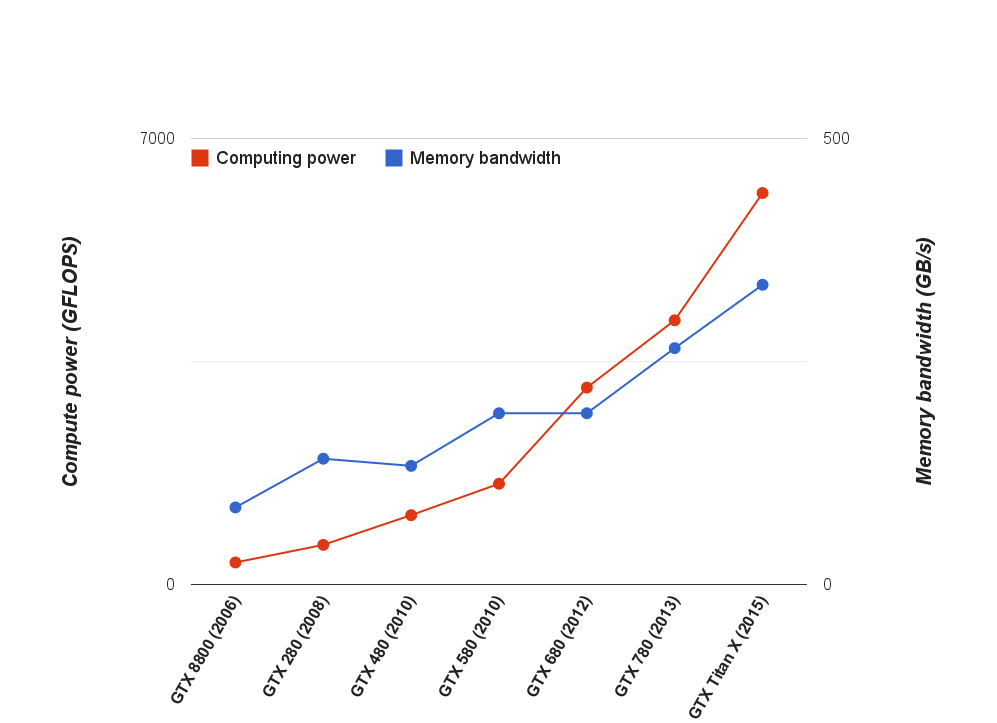
\includegraphics[scale=0.26]{computevsmemory.png}
\caption{\footnotesize\textnormal{Compute power and memory bandwidth over time/GPU generation.}}
\label{fig:compute-power}
\vspace{-0.4cm}
\end{figure}

Figure~\ref{fig:memsize} depicts how aggregate compute power and total size of fast on-chip memory (L1 cache and shared memory) have evolved over time.
The total amount of on-chip memory varies over time and at one point even decreases substantially from one generation to the next.
It has clearly not kept up with the increase in compute power. 

\begin{figure}[ht]
\center
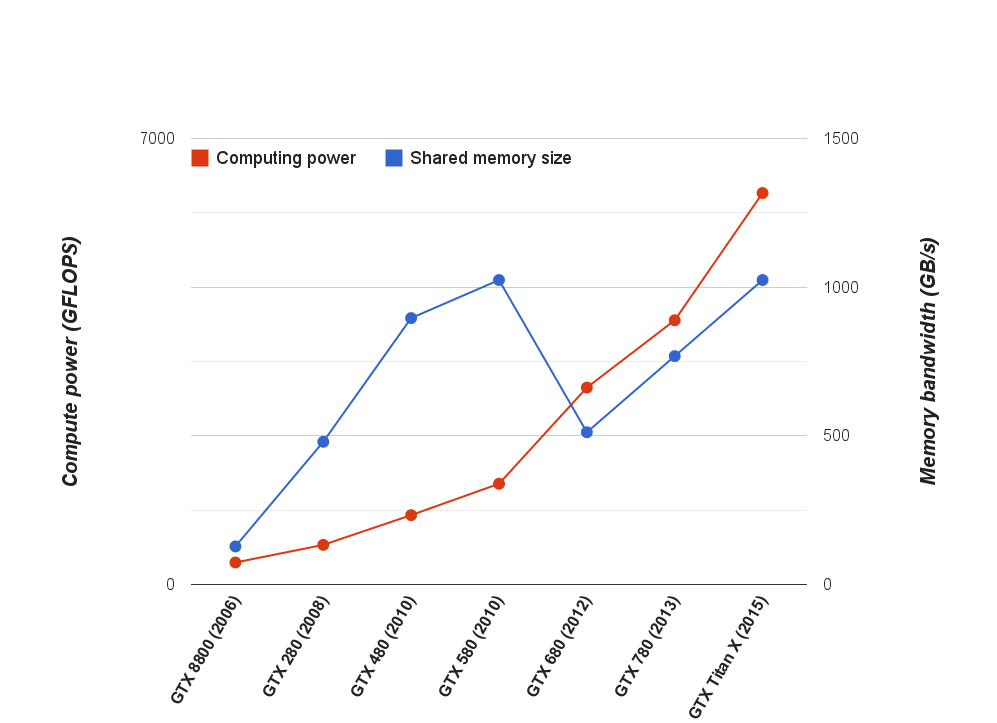
\includegraphics[scale=0.26]{computevsshared.png}
\caption{\footnotesize\textnormal{Compute power and  L1 / shared memory size over time/GPU generation.}}
\label{fig:memsize}
\vspace{-0.4cm}
\end{figure}

If these trends continue then the GPU cores will become increasingly memory starved.
Strategies to optimize GPU applications to make more efficient use of the memory hierarchy will likely become more important going forward.

Given the fact that future GPU generations may have smaller on-chip memory sizes, as has happened in
the past, GPU programmers cannot assume the availability of a specific shared memory size.
As a result, the programmer will need to design GPU applications so that they configure the use of
shared memory at run-time and possibly restrict the number of threads used by the application.
Or use run-time libraries, such as the one we are presenting in this paper, that automatically
adjust program behavior to the available hardware resources.

